\documentclass[a4paper,11pt]{article}
\usepackage{amsmath,amsthm,amsfonts,amssymb,amscd,amstext,vmargin,graphics,graphicx,tabularx,multicol} 
\usepackage[francais]{babel}
\usepackage[utf8]{inputenc}  
\usepackage[T1]{fontenc} 
\usepackage{pstricks-add,tikz,tkz-tab,variations}
\usepackage[autolanguage,np]{numprint} 

\setmarginsrb{1.5cm}{0.5cm}{1cm}{0.5cm}{0cm}{0cm}{0cm}{0cm} %Gauche, haut, droite, haut
\newcounter{numexo}
\newcommand{\exo}[1]{\stepcounter{numexo}\noindent{\bf Exercice~\thenumexo} : \marginpar{\hfill /#1}}
\reversemarginpar


\newcounter{enumtabi}
\newcounter{enumtaba}
\newcommand{\q}{\stepcounter{enumtabi} \theenumtabi.  }
\newcommand{\qa}{\stepcounter{enumtaba} (\alph{enumtaba}) }
\newcommand{\initq}{\setcounter{enumtabi}{0}}
\newcommand{\initqa}{\setcounter{enumtaba}{0}}

\newcommand{\be}{\begin{enumerate}}
\newcommand{\ee}{\end{enumerate}}
\newcommand{\bi}{\begin{itemize}}
\newcommand{\ei}{\end{itemize}}
\newcommand{\bp}{\begin{pspicture*}}
\newcommand{\ep}{\end{pspicture*}}
\newcommand{\bt}{\begin{tabular}}
\newcommand{\et}{\end{tabular}}
\renewcommand{\tabularxcolumn}[1]{>{\centering}m{#1}} %(colonne m{} centrée, au lieu de p par défault) 
\newcommand{\tnl}{\tabularnewline}

\newcommand{\trait}{\noindent \rule{\linewidth}{0.2mm}}
\newcommand{\hs}[1]{\hspace{#1}}
\newcommand{\vs}[1]{\vspace{#1}}

\newcommand{\N}{\mathbb{N}}
\newcommand{\Z}{\mathbb{Z}}
\newcommand{\R}{\mathbb{R}}
\newcommand{\C}{\mathbb{C}}
\newcommand{\Dcal}{\mathcal{D}}
\newcommand{\Ccal}{\mathcal{C}}
\newcommand{\mc}{\mathcal}

\newcommand{\vect}[1]{\overrightarrow{#1}}
\newcommand{\ds}{\displaystyle}
\newcommand{\eq}{\quad \Leftrightarrow \quad}
\newcommand{\vecti}{\vec{\imath}}
\newcommand{\vectj}{\vec{\jmath}}
\newcommand{\Oij}{(O;\vec{\imath}, \vec{\jmath})}
\newcommand{\OIJ}{(O;I,J)}


\newcommand{\bmul}[1]{\begin{multicols}{#1}}
\newcommand{\emul}{\end{multicols}}

\newcommand{\reponse}[1][1]{%
\multido{}{#1}{\makebox[\linewidth]{\rule[0pt]{0pt}{20pt}\dotfill}
}}

\newcommand{\titre}[5] 
% #1: titre #2: haut gauche #3: bas gauche #4: haut droite #5: bas droite
{
\noindent #2 \hfill #4 \\
#3 \hfill #5

\vspace{-1.6cm}

\begin{center}\rule{6cm}{0.5mm}\end{center}
\vspace{0.2cm}
\begin{center}{\large{\textbf{#1}}}\end{center}
\begin{center}\rule{6cm}{0.5mm}\end{center}
}



\begin{document}
\pagestyle{empty}
\titre{Interrogation : Proportionnalité et vitesse moyenne}{Nom :}{Prénom :}{Classe}{Date}

\exo{2,5}\\

\bmul{2}
\q Un grand magasin vend des agendas tous au même prix. A l'aide du produit en croix, trouver le prix x manquant dans le tableau suivant :\\

\columnbreak

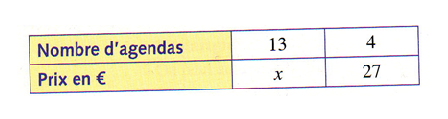
\includegraphics[scale=1]{tab1.eps} 

\emul

\noindent \reponse[2]\\

\q Avec 250 g de café, on peut préparer 32 expresso. \\
Quelle masse de café faut-il pour préparer 20 expresso ?\\
\reponse[3]\\

\q	Pour l'achat de 25 litres de carburant, Stéphanie a payé 27,50 euros. Quel est le prix de 40 litres ?\\
\reponse[3]\\

\exo{1} 
\bmul{2}
Le graphique ci-contre indique le prix de cinq ordinateurs en fonction de leur mémoire vive (exprimée en Mo).
Le prix est-il proportionnel à la mémoire vive de l'ordinateur? Expliquer.\\
\reponse[4]
\columnbreak

\includegraphics[scale=1]{pc.eps} 

\emul

\exo{3}

\bmul{2}
\initq \q Dans une banque parisienne, cinq clients désirant se rendre à Londres ont échangé le même jour des euros en livres Sterling. Les montants de leurs échanges sont reportés sur le graphique suivant :\\
\qa La somme en euros et en livres Sterling sont-elles proportionnelles ce jour là ? Expliquer.\\
\reponse[2]

\columnbreak

\includegraphics[scale=1]{exo.eps} 

\emul

\qa A l'aide du graphique et d'un tableau  de proportionnalité, donner, le plus précisément possible, la valeur de 150 euros en Livres.\\
\reponse[4]\\

\qa	A l'aide du graphique et d'un tableau de proportionnalité, donner, le plus précisément possible, la valeur de 140 Livres en euros.\\
\reponse[4]\\

\exo{2,5}

\initq 
\q En 2010, le marathon de Paris a été remporté chez les femmes par Tsede Baysa en 2 h 22 min. Cette course est longue de 42,195 km. Calculer la vitesse moyenne de Tsede Baysa durant cette course en km/h, puis en m/s. Arrondir au dixième.\\
\reponse[5]


\q Le TGV Eurostar traverse le tunnel sous la manche en 20 min à la vitesse moyenne de 160 km/h. Quelle est la longueur du tunnel? Arrondir au kilomètre.\\
\reponse[5]\\



\exo{1}
La vitesse du son dans l'air est de 340 m/s. A 6h30 du matin un volcan explose et émet un grondement. Au bout de combien de temps les habitant d'une ville située à 25 km vont-ils entendre le grondement ?\\
\reponse[4]\\


\end{document}
